\documentclass{beamer}
\usepackage{graphicx}
\usepackage{times}
\usepackage[polish]{babel}
\usepackage{polski}
\usepackage[utf8]{inputenc}

% dodatkowe pakiety
\usepackage{enumerate}
% Listings ------------------------------------------------------------
\usepackage{listings}
% Scala listings
% "define" Scala
\lstdefinelanguage{scala} {
  morekeywords={abstract,case,catch,class,def,%
    do,else,extends,false,final,finally,%
    for,if,implicit,import,match,mixin,%
    new,null,object,override,package,%
    private,protected,requires,return,sealed,%
    super,this,throw,trait,true,try,%
    type,val,var,while,with,yield},
  otherkeywords={=>,<-,<\%,<:,>:,\#,@},
  sensitive=true,
  morecomment=[l]{//},
  morecomment=[n]{/*}{*/},
  morestring=[b]",
  morestring=[b]',
  morestring=[b]"""
}

% IntelliJ Colors for listings
\usepackage{color}
\definecolor{dkgreen}{rgb}{0,0.6,0}
\definecolor{gray}{rgb}{0.5,0.5,0.5}
\definecolor{mauve}{rgb}{0.58,0,0.82}
 
% Default settings for code listings
\lstset{
  frame=tb,
  language=Scala,
  aboveskip=3mm,
  belowskip=3mm,
  showstringspaces=false,
  columns=flexible,
  basicstyle={\small\ttfamily},
  numbers=none,
  numberstyle=\tiny\color{gray},
  keywordstyle=\color{blue},
  commentstyle=\color{gray},
  stringstyle=\color{dkgreen},
  frame=single,
  breaklines=true,
  breakatwhitespace=true
  tabsize=2
}

% \lstloadlanguages{TeX}

\usetheme{AGH}

\title[\textbf{ProtoDoc} - odpowiednik JavaDoc dla Google ProtoBuf]{ProtoDoc - \\ odpowiednik JavaDoc\\ dla Google Protocol Buffers}

\author[K. Malawski]{Konrad Malawski}

\date[2011]{6-12-2011}

\institute[AGH]
{Wydział Elektrotechniki, Automatyki, Informatyki i Elektroniki\\ Katedra Automatyki}

\setbeamertemplate{itemize item}{$\maltese$}

\begin{document}

%---------------------------------------------------------------------------


{
\usebackgroundtemplate{
\includegraphics[width=\paperwidth]{titlepage}} % wersja angielska
%\usebackgroundtemplate{
\includegraphics[width=\paperwidth]{titlepagepl}} % wersja polska
 \begin{frame}
   \titlepage
 \end{frame}
}

%---------------------------------------------------------------------------


\begin{frame}
\frametitle{Plan prezentacji}
 \begin{itemize}
  \item Wprowadzenie
         \begin{itemize}
          \item Przedstawienie problemu dokumentacji Protocol Buffers
	  \item Cel projektu
         \end{itemize}

  \pause \item Opis implementacji
	 \begin{itemize}
	  \item Architektura aplikacji
	  \item Porównanie narzędzi i uzasadnienie dokonanych wyborów
	  \item Scala Parser Combinators
	 \end{itemize}
  
   \pause \item Wyniki pracy
         \begin{itemize}
          \item Integracja z Apache Maven
          \item Przykładowy efekt działania aplikacji
         \end{itemize}
  \pause \item Podsumowanie i przyszłość projektu
 \end{itemize}
\end{frame}

%---------------------------------------------------------------------------


\begin{frame}
\frametitle{Problemy dokumentacji Protocol Buffers}
Nie istnieje zunifikowany sposób dokumenowania oraz publikowania wiadomości Protocol Buffers. \\  
\_ \\ 

Typowymi problemami są:
 \begin{itemize}
  \pause \item Praca z wygenerowanymi z ProtoBuf klasami, \\
               nie zawierającymi dokumentacji.
  \pause \item Trudności w rozpoznawaniu pól ,,legacy'', których nie powinno się już używać. \\
               (Raz dodane do wiadomości pole, zostaje w niej ,,na zawsze'').
  \pause \item Brak możliwości przeglądnięcia dokumetacji / listy wiadomości online (przed pobraniem ich).
 \end{itemize}

\end{frame}

%---------------------------------------------------------------------------


\begin{frame}
\frametitle{Cel projektu}

\textbf{ProtoDoc} stawia sobie za cel rozwiązanie problemów dokumentowania wiadomości Protocol Buffers poprzez:
\begin{itemize}
 \pause \item Parsera języka definicji interfejsów Protocol Buffers (pliki *.proto)
        \begin{itemize}
         \item Nie ignorując komentarzy.
        \end{itemize}

 \pause \item Stworzenie narzędzia generującego z uzyskanych informacji stronę www (ala JavaDoc), 
       zawierającą wszystkie wiadomości jak i ich komentarze, pola oraz definiowane typy.
\end{itemize}

\end{frame}

%---------------------------------------------------------------------------


\begin{frame}[fragile]
\frametitle{Architektura aplikacji}
\begin{center}
 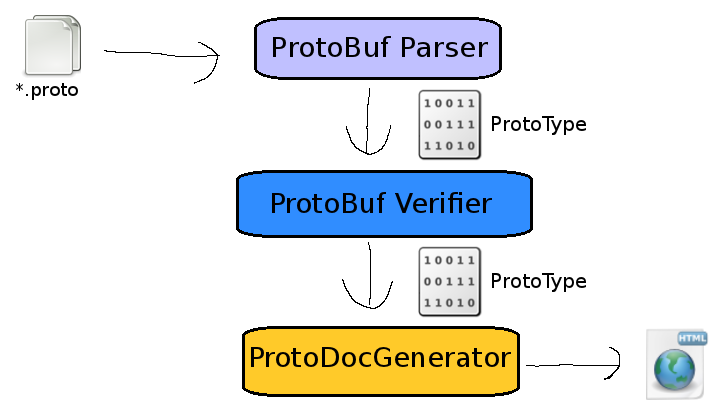
\includegraphics[scale = 0.45]{protodoc_flow}
 % protodoc_flow.png: 398x738 pixel, 93dpi, 10.87x20.16 cm, bb=0 0 308 571
\end{center}
\end{frame}

%---------------------------------------------------------------------------


\begin{frame}[fragile]
\frametitle{Architektura aplikacji}
\begin{itemize}
 \item ProtoBuf\textbf{Parser}
 \begin{itemize}
  \item Parsuje po jednym pliku (który może zawierać wiele wiadomości)
  \item Tworzy obiektu typu ProtoType, zawierające pełną informację o typie / wiadomości
  \item Przeprowadza analizę syntaktyczną
 \end{itemize}

 \pause \item ProtoBuf\textbf{Verifier}
 \begin{itemize}
  \item Uruchamiany jest po zakończeniu parsingu wszystkich plików
  \item Przeprowadza \textbf{analizę semantyczną} uzyskanych obiektów \textit{ProtoType}
  \item Między innymi, sprawdza widoczność oraz poprawność używanych typów
 \end{itemize}

 \pause \item ProtoDoc\textbf{Generator}
 \begin{itemize}
  \item Generuje strony www zawierające informacje o sparsowanych wiadomościach (\textit{ProtoType}'ach)
  \item Wykorzystuje również informacje o potencjalnych błędach które mógł wykryć \textbf{ProtoBufVerifier}
 \end{itemize}

\end{itemize}

\end{frame}

%---------------------------------------------------------------------------


\begin{frame}
\frametitle{Wybór narzędzia implementacji parsera}
Podczas wyboru technologii (generatora) parsera przeglądano popularne narzędzia takie jak JBison / JFlex,
jednak ostateczny wybór padł na Scala Parser Combinators - z powodu elegancji tego rozwiązania.\\

\pause
\begin{block}{Kombinator Parserów}
 Podejście to pozwala na czytelną i elegancką implementację Rekursywnie Zstępującego Parsera.
\end{block}

% http://en.wikipedia.org/wiki/Parser_combinator
\end{frame}

%---------------------------------------------------------------------------


\begin{frame}
\frametitle{Scala Parser Combinators}
Kombinatory parserów (konkretna implementacja) są częścią języka \textbf{Scala}, zastosowanego do implementacji parsera w tym projekcie. \\
\_ \\

Zalety zastosowanego rozwiązania:
\begin{itemize}
 \pause \item Kod jest czytelny oraz łatwy w utrzymaniu (przypomina notację BNF)
 \pause \item Nie jest konieczne generowanie plików ,,implementacji'' parsera, definicje które piszemy same z siebie są wykonywalne
 \pause \item Umożliwia to podejście do projektu w sposób \textbf{prowadzony testami} (ponad 40!).
\end{itemize}


% \begin{columns}
% \column{0.45\textwidth}
%  \begin{block}{Za:}
%   \begin{itemize}
%    \item 
%   \end{itemize}
% 
%  \end{block}
% 
% \column{0.45\textwidth}
%  \begin{block}{Przeciw:}
%   
%  \end{block}
% \end{columns}

\end{frame}

%---------------------------------------------------------------------------


\begin{frame}[fragile]
\frametitle{Integracja z Apache Maven}
Analogicznie jak w przypadku znanego pluginu \textbf{JavaDoc}:

% \textbf{JavaDoc:}
\begin{lstlisting}
mvn javadoc:javadoc
\end{lstlisting}

\textbf{ProtoDoc:}
\begin{lstlisting}
mvn protodoc:protodoc
\end{lstlisting}

\begin{center}
 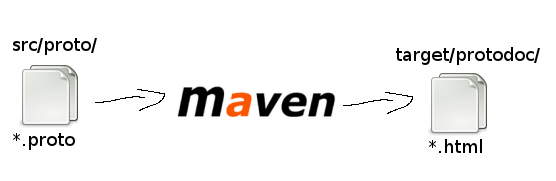
\includegraphics[scale = 0.40]{maven_files_flow}
 % maven_files_flow.png: 556x181 pixel, 90dpi, 15.69x5.11 cm, bb=0 0 445 145
\end{center}

\end{frame}

%---------------------------------------------------------------------------


\begin{frame}
\frametitle{Przykładowy efekt działania aplikacji}
\begin{center}
 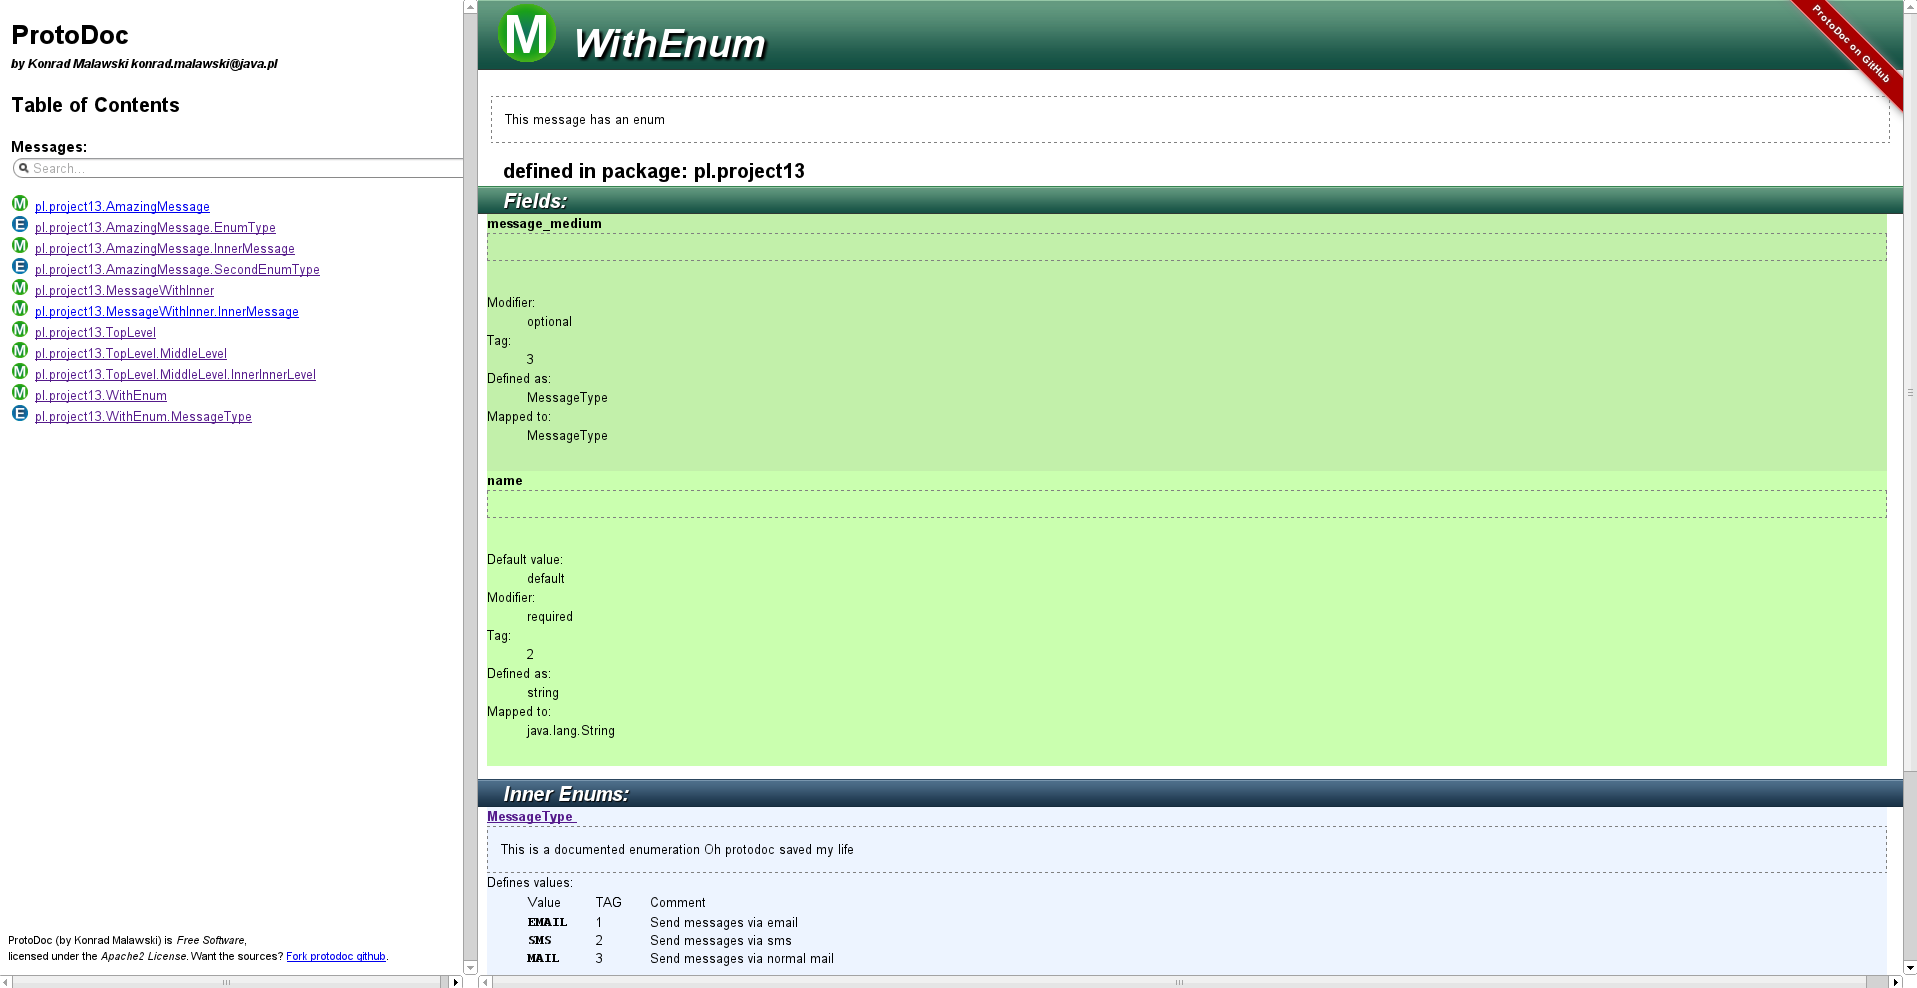
\includegraphics[width = \textwidth]{protodoc_msg}
 % protodoc_msg.png: 1917x988 pixel, 93dpi, 52.36x26.99 cm, bb=0 0 1484 765
\end{center}
\end{frame}

%---------------------------------------------------------------------------


\begin{frame}
\frametitle{Przykładowy efekt działania aplikacji}
\begin{center}
 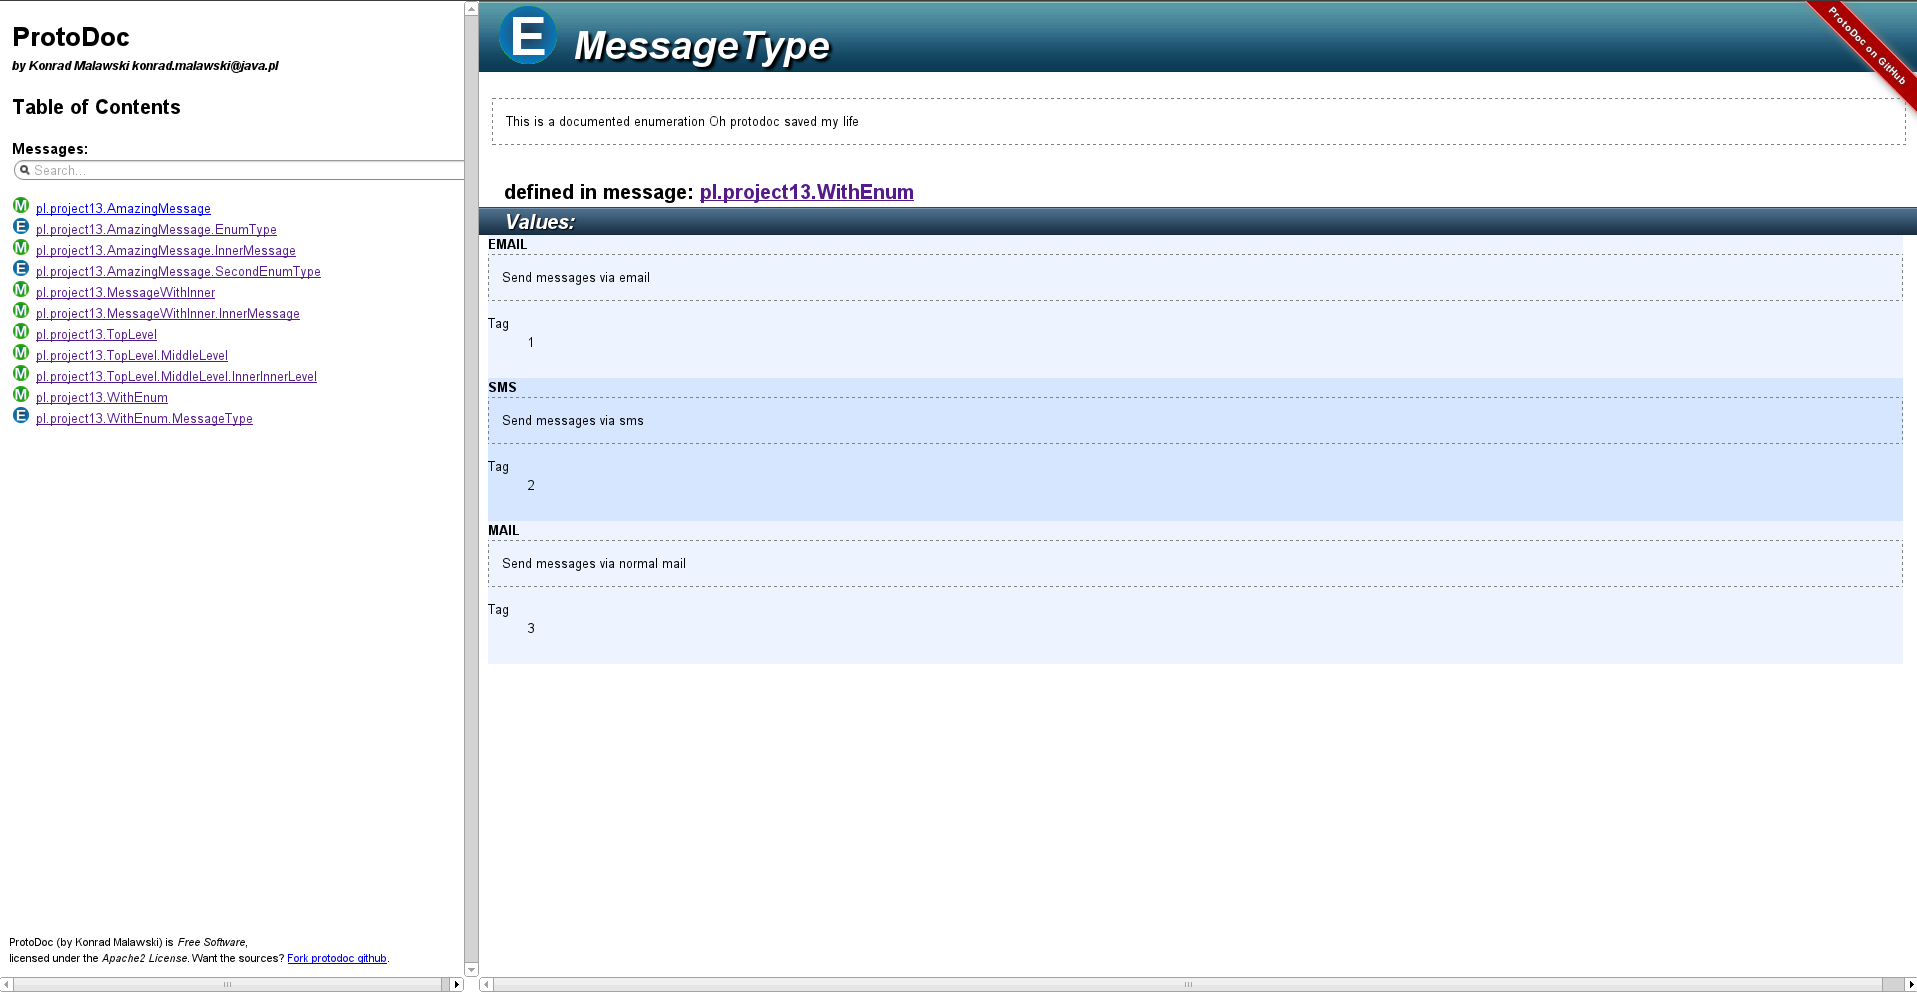
\includegraphics[width = \textwidth]{protodoc_enum}
 % protodoc_enum.png: 1917x988 pixel, 93dpi, 52.36x26.99 cm, bb=0 0 1484 765
\end{center}
\end{frame}

%---------------------------------------------------------------------------


\begin{frame}
\frametitle{Podsumowanie i przyszłość projektu}
Spełniono założenia projektu.

Powstał:
 \begin{itemize}
  \item Parser podstawowej części Protocol Buffers Interface Description Language
  \item Generator dokumentacji
  \item \small{... jako element dodatkowy element} - Weryfikator poprawności (widoczności typów) w sparsowanych wiadomościach
 \end{itemize}

\end{frame}

%---------------------------------------------------------------------------


\begin{frame}
\frametitle{Przyszłość projektu}
\begin{itemize}
 \item Plugin Mavenowy zostanie opublikowany w \textbf{Maven Central} \\
       \small{Umożliwiając dowolne wykorzystywanie go ,,out of the box''} w rzeczywistych projektach.
 \item \textbf{Plugin jak i parser} zostaną umieszczone na ogólnodostępnej stronie www,
       pod licencją GPLv3, celem ułatwienia wprowadzania poprawek przez społeczność.
\end{itemize}

\end{frame}


%---------------------------------------------------------------------------


\begin{frame}
\frametitle{Dziękuję za uwagę}

\begin{center}
 \LARGE{Dziękuję za uwagę.} 
\end{center}


\end{frame}


\end{document}

